\chapter{Classificação utilizando aprendizado profundo}

O capítulo anterior tratou-se de uma solução baseada em seleção de candidatos, extração de características e posterior classificação, o que caracteriza uma técnica superficial. Nesse capítulo propomos uma solução híbrida, que utiliza a seleção de candidatos idêntica à anterior, porém utiliza técnicas profundas de classificação de modo que os candidatos são diretamente inseridos no classificador. Inicialmente introduz-se as redes MLP e convolucionais, fornecendo as bases teóricas, funções de ativação e processo treinamento.  Questões relativas à implementação também são abordadas.

\section{Perceptron Multicamadas (MLP)}

Segundo \cite{DLbook}, uma rede de perceptrons multicamadas (MLP) também pode ser chamada de rede profunda sem realimentação (\textit{deep feedforward networks}), também chamada de rede neural, e tem como objetivo aproximar uma função $f^*$. Para o problema de classificação, $y=f^*(x)$, onde $y$ é a categoria e $x$ a amostra, a rede define um mapeamento $y = f(x,\theta)$, onde $\theta$ são os parâmetros do modelo. O problema consiste em encontrar $\theta$ que resulte na melhor aproximação de $f^*$.

Essa estrutura é chamada de rede pois são representadas como um conjunto de camadas, cada uma alimentando a próxima, o que gera uma cadeia de funções: $y=f^1(f^2(f^3(x)))$, cada qual representando uma camada. Além disso, não ocorre alimentação pois a informação flui continuamente através das camadas desde a entrada $x$ sequencialmente até a camada de saída $y$.

Parte-se de um modelo linear simples,
\begin{equation}
y=w^Tx+b
\end{equation}
em que $w$ corresponde ao vetor de pesos do classificador e $b$ bias. Verifica-se que esse modelo pode ser treinado de maneira simples e rápida, porém serve apenas para casos em que o dataset é linearmente separável, diferente da maioria dos problemas reais. Como visto na seção \ref{sec:classificacao:svm}, técnicas de mapeamento não lineares $\phi(x)$ são alternativas para tentar tornar essas amostras linearmente separáveis, como é o caso da função RBF. Na abordagem superficial, deve-se escolher esse mapeamento de maneira específica às amostras de forma manual. 

Advém, então, uma das principais contribuições dos métodos profundos: a função de mapeamento $\phi(x,\theta)$ é determinada, entre uma gama ampla de funções, pelo próprio sistema através dos parâmetros $\theta$. Isso pode ser interpretado como a seleção automática, pelo algoritmo, do extrator de características que melhor representa o dataset. Assim, o modelo se torna 
\begin{equation}
y=f(x,\theta,w) = w^T\phi(x,\theta)
\end{equation}
Na rede, $\phi$ corresponde às camadas intermediárias. Os parâmetros $w$ mapeiam, então, o resultado da camada intermediária $\phi(x,\theta)$, que representam as descrições da amostra, para a camada de saída $y$. O princípio de aprender o extrator características mais apropriado para o dataset não é exclusivo para redes MLP e se aplica a outros modelos de aprendizado profundo.

Nota-se, ainda, que no caso mais geral, para camadas de saída com funções de ativação não lineares, teríamos o modelo generalizado
\begin{equation}
y=f(x,\theta,w,b) = \gamma(w^T\phi(x,\theta)+b)
\end{equation}
onde $\gamma(x)$ é a função de ativação da camada de saída.

\section{Função de ativação}
Como visto na seção \ref{introducao:perceptron}, os perceptrons aplicam uma função de ativação ao somatório ponderado das entradas. A escolha dessa função está associada à interpretação que se dá à saída. Duas funções foram utilizadas nesse trabalho e serão introduzidas a seguir.

\subsection{Sigmoide}
Como visto anteriormente, a escolha da função relaciona-se com a interpretação do valor de saída. Para classificadores interpreta-se o valor dos perceptrons da camada de saída como probabilidades da amostra pertencer a uma determinada classe. Nesse caso espera-se que esses valores estejam no intervalo $[0,1]$. Uma função que assegura essa condição é a sigmoide
\begin{equation}
	\label{eq:sigm}
	\sigma(x) = \frac{1}{1+e^{-x}}
\end{equation}

\begin{figure}[h]
\centering
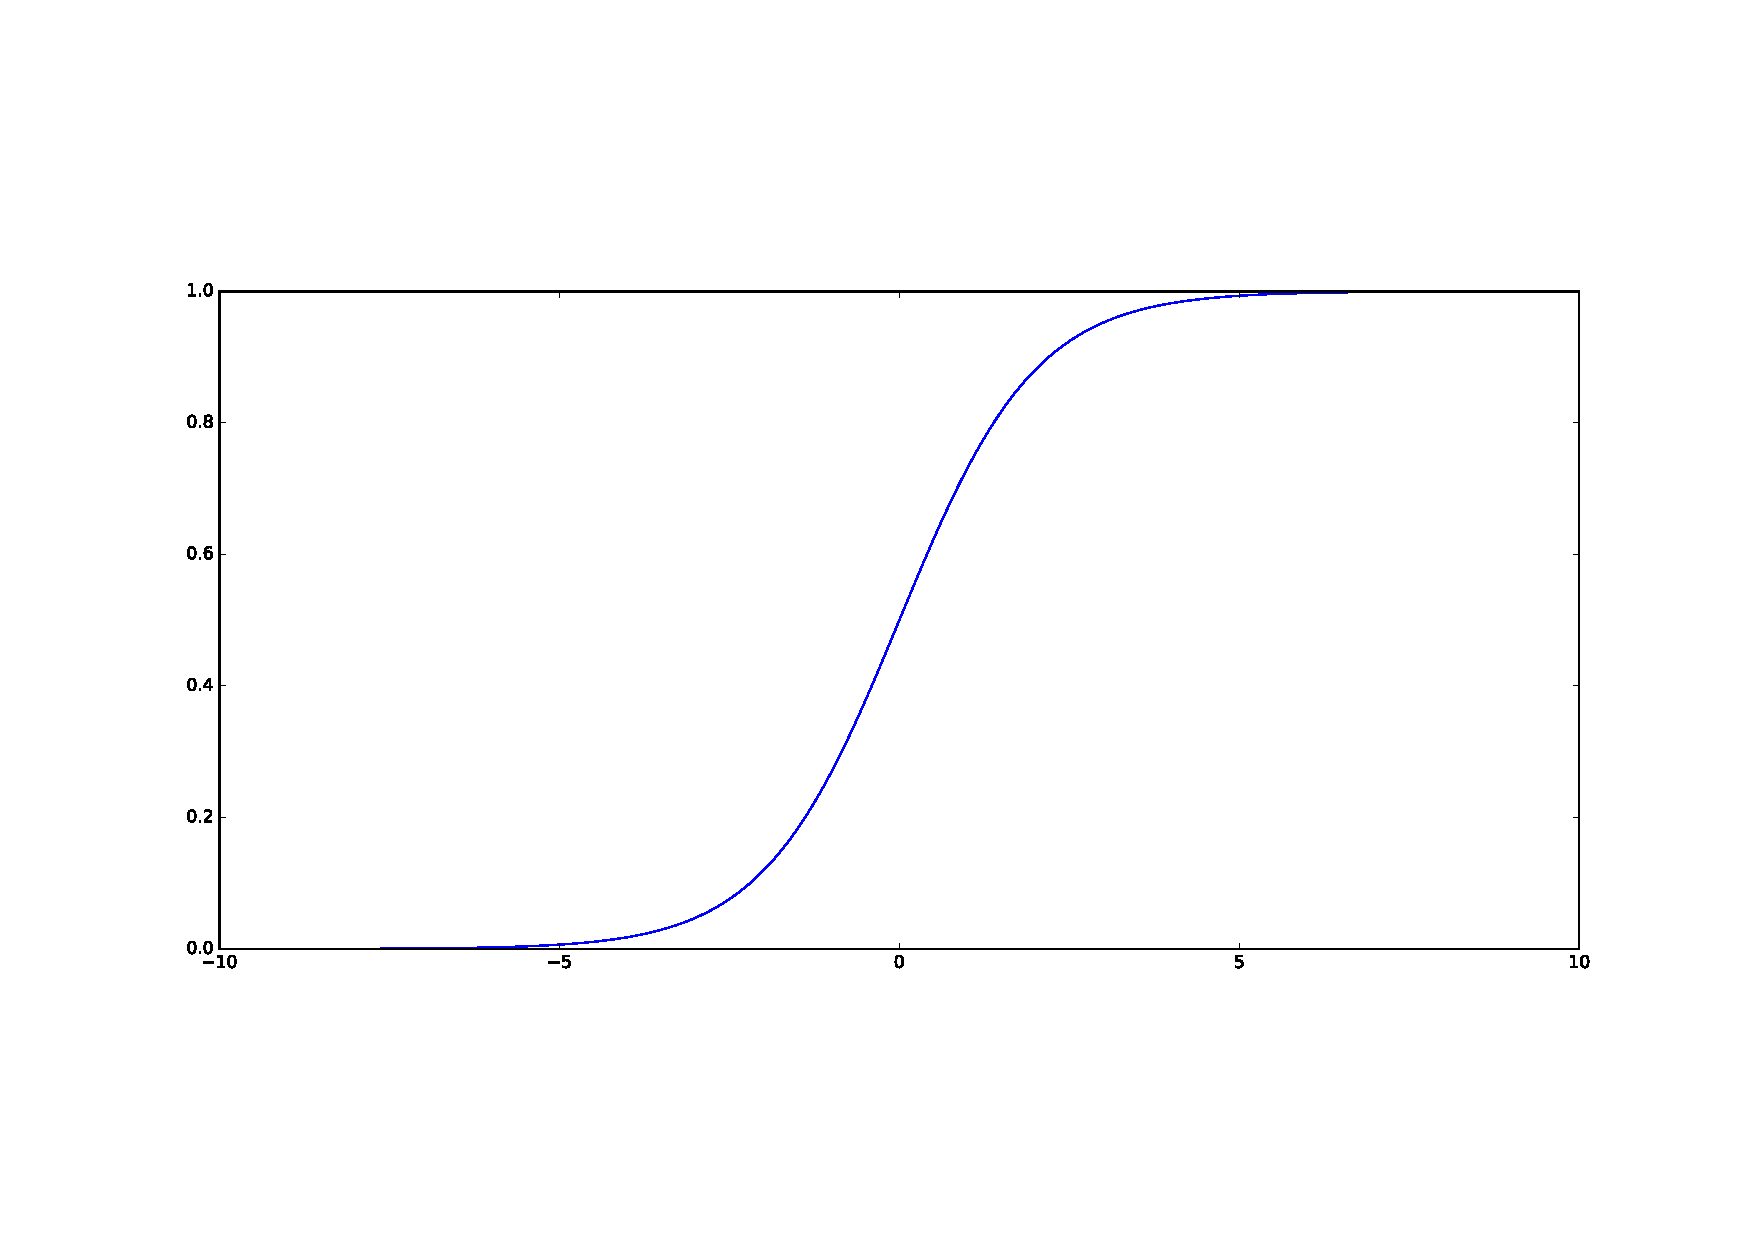
\includegraphics[width=0.9\textwidth]{deep/sigmoid}
\caption{Gráfico mostrando o comportamento da sigmoide}
\label{fig:sigmoid}
\end{figure}

Outra característica importante é a não linearidade da função que permite transformar conjuntos não linearmente separáveis. Por outro lado, observa-se que essa função satura facilmente com entradas pŕoximas de 1 ou 0, ocasionando uma derivada praticamente nula nessas regiões. Como será visto adiante isso é um problema ao se considerar que a derivada dessa função definirá a atualização dos pesos desses perceptrons durante o processo de treinamento. Ao propagar esse processo camada a camada, verificam-se derivadas cada vez menores, o que causa o problema do gradiente enfraquecido, em que as camadas iniciais não conseguem aprender pois o gradiente é muito reduzido.

\subsection{RELU}
Para resolver o problema do gradiente enfraquecido a \textit{Rectified Linear Unit -- RELU} foi proposta \cite{nair2010relu} como
\begin{equation}
	\label{eq:relu}
	\text{RELU}(x) = \max\{0,x\}
\end{equation}

Observa-se que para valores positivos essa função tem uma derivada constante e igual a um, proporcionando um gradiente considerável sempre que o perceptron estiver ativo. Por outro lado, para valores negativos considera-se o perceptron inativo e os pesos não são atualizados. Ao mesmo tempo essa característica garante a não linearidade da função.

\section{Treinamento}
O processo de treinamento de uma rede neural é um problema de otimização. Porém, diferentemente do caso do SVM, trata-se de uma otimização não convexa, isto é, existem múltiplos mínimos locais para a função custo e diversas soluções podem ser encontradas, dependendo dos valores iniciais dos parâmetros. Esse fato advém do caráter não linear das funções de ativação nas camadas intermediárias que irão definir a extração de características.

Durante essa etapa otimiza-se os parâmetros $\theta$ de forma que $y \approx f^*(x)$. Isso é feito através da minimização de uma função custo $C(\theta)$ por um algoritmo de otimização chamado SGD utilizando o gradiente de $C$ obtidas por um algoritmo de propagação reversa de erros. Todos esses passos são descritos a seguir.

\subsection{Função custo}
A função custo quantifica a qualidade de representação que o modelo oferece para o conjunto de treinamento, isto é, qual a medida de erro que o classificador comete dentro do próprio conjunto de treinamento. Duas funções custos utilizadas na implementação são apresentadas a seguir.

Em geral podemos escrever a função custo como
\begin{equation}
C(\theta) = \sum_{x \in \text{dataset}} C_x
\end{equation}
de forma que podemos calcular o custo de cada amostra, nessa seção representada pelo par $(x,y)$, individualmente, correspondente ao erro equivalente àquela amostra.

Uma função usual e que tem uma noção intuitiva forte é a média dos erros quadráticos -- MSE:
\begin{equation}
\label{eq:mse}
C(\theta) = \frac{1}{n} \sum_{x_1 \ldots x_n} \left(y - f(x,\theta)\right)^2
\end{equation}
Nessa função fica evidenciado o cálculo do erro como a distância quadrática entre a categoria determinada pelo modelo e a verdadeira. Quando o modelo apresenta a mesma categoria especificada mediante treinamento para todas as amostras verifica-se um custo nulo.

A escolha da função custo está associada também à função de ativação da camada de saída. Isso é importante pois no caso de uma ativação sigmoide a saída satura rapidamente, o que provoca uma derivada muito pequena e, como veremos adiante, impossibilita atualização dos parâmetros da rede. Para esse fim, introduz-se a função custo de entropia cruzada binária (\textit{binary cross entropy}) descrita por
\begin{equation}
\label{eq:bcr}
C(\theta) = -\frac{1}{n} \sum_{x_1 \ldots x_n} \left[y \ln f(x,\theta) + (1-y) \ln (1-f(x,\theta))\right]
\end{equation}
cuja grande contribuição é permitir o uso de unidades sigmoidais na camada de saída sem que ocorra um gradiente baixo, visto que a função exponencial da ativação é revertida ao se utilizar o logaritmo natural imposto pela entropia cruzada. Nota-se ainda, no caso em que $f(x,\theta)=y=m$ de maneira que $m \in {0,1}$, temos um custo nulo dessa função.

Tendo uma métrica para avaliar a qualidade do classificador em relação ao dataset utiliza-se um algoritmo de otimização para encontrar parâmetros que melhorem o desempenho desse mecanismo.

\subsection{\textit{Stocastic Gradient Descent} -- SGD}
Um método tradicional para minimização é o do gradiente descendente, que utiliza a aproximação
\begin{equation}
\Delta C \approx \pd{C}{w} \Delta w \pd{C}{b} \Delta b = \nabla C \cdot \Delta \theta
\end{equation}
para verificar a variação $\Delta C$ na função custo em função da variação nos parâmetros de $\Delta w$ e $\Delta b$. Basicamente escolhe-se os parâmetros inicialmente aleatórios e então busca-se encontrar o vetor de variação dos parâmetros $\Delta \theta = (\Delta w, \Delta b)^T$ que façam C diminuir. Se escolhermos $\Delta \theta = -\eta \nabla C$, teremos
\begin{equation}
\Delta C = -\eta \abs{\nabla C}^2
\end{equation}
que será negativo ao escolhermos $\eta > 0$, chamado de taxa de aprendizado (\textit{learning rate}). Esse processo é executado iterativamente, atualizando os parâmetros com $\theta \gets \theta + \Delta \theta$ até se encontrar um mínimo local.

Em geral redes profundas necessitam de um grande número de amostras para serem treinadas. O cálculo do gradiente $\nabla C$ é custoso ao se considerar a quantidade amostras, visto que $\nabla C = \sum_x \nabla C_x$. Utiliza-se, então, uma variação do método chamada de \textit{Stochastic Gradient Descent} -- SGD. Essa variação divide o dataset em subconjuntos aleatórios $M$ chamados \textit{mini batches} e estima o gradiente fazendo a soma dos gradientes individuais apenas nesses subconjuntos a cada iteração do método, o que reduz drasticamente o tempo de execução do algoritmo.
\begin{equation}
\nabla C \approx \sum_{x \in M} \nabla C_x
\end{equation}

\subsection{Backpropagation}
%neuralnetworksanddeeplearning.com/chap2.html

O método de otimização anterior faz uso do gradiente de função custo $\nabla C$, porém não mostra como calcular essa quantidade. Para isso é necessário encontrar as derivadas da função custo em relação aos pesos individuais de cada elemento da rede, $w$ e $b$. De fato, utilizar as ferramentas do cálculo se mostra um desafio na prática, visto a complexidade da função custo em termos da função da rede $f(x, \theta)$ que combina todas as não linearidades encadeadas nas camadas. 

Uma solução foi o algoritmo de propagação reversa de erros (\textit{backpropagation}), já existente na década de 1979 porém proposto mais recentemente em \cite{backpropagation}, que fornece um método eficiente de calcular as derivadas da função custo em relação a quaisquer parâmetros $w$ e $b$ da rede.

Primeiramente formaliza-se a notação utilizada. Convenciona-se $w_{jk}^l$ como o peso da conexão entre o perceptron $j$ da camada $l$ a o perceptron $k$ da camada $(l-1)$, como ilustrado na figura \ref{fig:bp}. De maneira semelhante, $b^l_j$ e $a^l_j$ indicam o bias e a ativação do perceptron $j$ da camada $l$ com
\begin{equation}
a^l_j = \sigma (z^l_j) =\sigma \left( \sum_k w_{jk}^l a_k^{l-1} + b_j^l \right)
\end{equation}
onde $\sigma(x)$ é a função de ativação da rede. Define-se também uma grandeza intermediária chamada de erro da camada $l$, $\delta^l$, interpretada como a contribuição da camada $l$ para o erro total, através do qual serão calculadas as grandezas de interesse.

\begin{figure}[ht]
\centering
\begin{subfigure}{.5\textwidth}
  \centering
  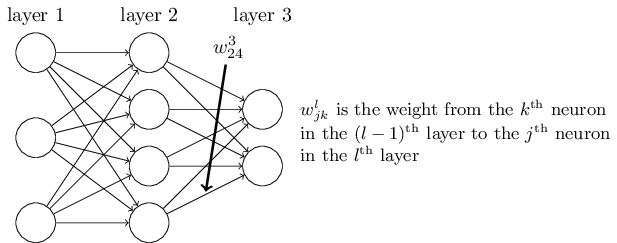
\includegraphics[width=\linewidth]{deep/bp-weights}
\end{subfigure}%
\begin{subfigure}{.5\textwidth}
  \centering
  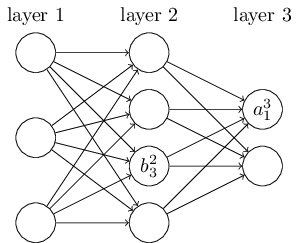
\includegraphics[width=0.8\linewidth]{deep/bp-bias}
\end{subfigure}
\caption{Conveção das conexões entre perceptrons}
\label{fig:bp}
\end{figure}

Esse algoritmo possui uma formulação complexa que não está no escopo desse trabalho. Entretanto, alguns aspectos serão enfatizados pela análise simples das equações fornecidas por esse método, vistas a seguir.

\begin{align}
\delta^L &= \nabla_a C \odot \sigma^\prime(z^L) \\ 
\delta^l &= ((w^{l+1})^T\delta^{l+1}) \odot \sigma^\prime(z^l) \\
\pd{C}{b_j^l{}} &= \delta_j^l \\ 
\pd{C}{w_{jk}^l{}} &= a_k^{l-1} \delta_j^l 
\end{align}

Pode-se entender o algoritmo como calculando o erro na camada de saída, $\delta^L$ e propagando esse erro para as outras camadas, obtendo os correspondentes $\delta^l$ através dos quais as demais derivadas são obtidas e permitem obter o gradiente da função custo. 

Um aspecto a destacar é o papel fundamental da derivada da função de ativação $\sigma(x)$. Se ela saturar, essa derivada terá um valor baixo, o que provoca um gradiente pequeno e a atualização dos parâmetros fica estagnada, impedindo o aprendizado. Por isso a importância de funções de ativação que impedem a saturação, como a RELU, vista anteriormente.

Similarmente, a última equação mostra que a derivada da função custo em relação ao pesos de um determinado perceptron é proporcional à entrada correspondente ào perceptron de entrada. Portanto, caso a entrada seja nula, essa componente do gradiente será também nula, o que significa que o perceptron só tem seu peso atualizado quando estiver ativo.

\section{Redes convolucionais}
%http://neuralnetworksanddeeplearning.com/chap6.html#introducing_convolutional_networks

A estrutura MLP vista anteriormente é chamada de completamente conectada, onde cada perceptron em uma camada está conectado à todos os perceptrons da próxima camada. Uma variante desse modelo são as chamadas redes convolucionais, que introduzem um aspecto espacial no processamento das amostras de forma que as camadas possuam uma estrutura. São especialmente úteis para amostras de maior dimensão que têm uma estrutura matricial, como imagens. Se destacam em relação à MLP pois a relação de estrutura não precisa ser incorporada ao modelo via treinamento mas já advém diretamente do modelo utilizado.

Apesar de já existirem na década de 1970 considera-se que o trabalho \cite{lecun1998convnet} foi fundamental para estabelecer a teoria moderna das redes convolucionais. Essas redes continuam organizadas em camadas, porém não são completamente conectadas. Conectam-se as camadas através dos chamados campos receptivos locais (\textit{local receptive fields}) que ligam uma série de perceptrons da camada anterior à próxima, como vistos na figura \ref{fig:convnet-receptivefield}. Os campos receptivos são transladados para obter as conexões dos próximo perceptrons na camada intermediária.

\begin{figure}[h]
\centering
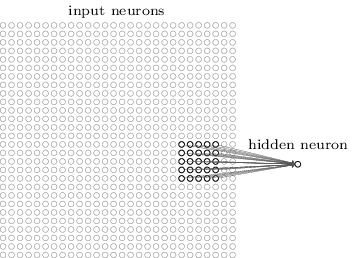
\includegraphics[width=0.5\textwidth]{deep/convnet-receptivefield}
\caption{Exemplo de rede convolucional e campos receptivos.}
\label{fig:convnet-receptivefield}
\end{figure}

Além desse aspecto de estrutura introduzido pelos campos receptivos, tem-se que os pesos e bias são compartilhados pelos diferentes campos receptivos. Isto é, para cada perceptron da camada intermediária embora as ligações ocorram com diferentes perceptrons da camda anterior, elas compartilham o mesmo peso e isso reduz drasticamente a quantidade de parâmetros da rede, tornando o precesso de treinamento mais rápido. Portanto tem-se que os diferentes campos receptivos são sensíveis à um mesmo padrão ou característica (\textit{feature}) e isso garante uma invariância à translação. Os pesos compartilhados são também chamados de núcleo (\textit{kernel}). De fato, observa-se que essa operação é resumida como uma convolução entre a camada anterior e o núcleo:
\begin{equation}
a^1 = \sigma(b+ w \ast a^0) 
\end{equation}
onde $a^0$ é a camada anterior e $a^1$ o primeiro mapa de características, sendo $\sigma(x)$ a função de ativação e $w$ o núcleo.

Na prática, entretanto, utilizam-se múltiplos núcleos de maneira a obter um mapa de características mais rico. Isso significa aumentar drasticamente a dimensionalidade da rede. Isso implica na necessidade de utilizar camadas de \textit{pooling} que reduzem a dimensionalidade da rede através de uma amostragem. Uma das possibilidades é utilizar \textit{max-pooling}, uma técnica não linear que implica selecionar a maior amostra dentro da região. Basicamente condensa-se a informação sobre a característica que se deseja encontrar sem se preocupar com sua localização exata. Atenta-se para o fato de que essa operação é realizada para cada mapa de características isoladamente.

Por fim, após camadas convolucionais e de amostragem, tem-se mapas de características densos que possibilitam à camada densamente conectadas consecutivas fazer o processo final de classificação, como ilustrado na figura \ref{fig:convnet}. 

O processo de treinamento é similar às MLPs, porém com pequenas modificações dado o caráter estrutural e convolucional da rede.

\section{Implementação}
A solução híbrida proposta nesse capítulo assume que os candidatos são obtidos através do algoritmo tradicional visto na seção \ref{sec:tradicional-candidatos} e utiliza um classificador profundo sem que haja pré-processamento das amostras. Dois tipos de estruturas foram utilizadas, primeiramente uma rede MLP e em seguida uma rede convolucional.

Existem diversas plataformas para se implementar os métodos de redes neurais. Entre essas, destacam-se a biblioteca de código aberto \textsc{Theano} \cite{theano}, que permite a definição de e avaliação de expressões matemáticas multidimensionais, diferenciação simbólica, otimização para velocidade e estabilidade, além de uso transparente da GPU. Essa biblioteca, entretanto, não fornece funções específicas para a criação de redes neurais, ou seja, é necessário que o usuário crie as matrizes de pesos, defina função custo e de ativação.

Para facilitar a utilização dos métodos profundos e tornar o processo de desenvolvimento mais rápido, utilizou-se a a biblioteca \textsc{Keras} \cite{keras}, que fornece uma abstração acima do \textsc{Theano} para utilização dos métodos profundos. Isso permite criar redes com poucas linhas de código, definindo camadas de maneira simples e escolhendo as funções de ativação e custo dentre as já definidas. Ainda assim, permite flexibilidade para o usuário criar suas próprias funções e ajustar parâmetros da rede, assim como métodos de iniciação dos parâmetros e diferentes tipos de otimizadores.

Ambas as bibliotecas são desenvolvidas para \textsc{Python} e portanto houve a necessidade de integrar esse código ao já existente em C++. Destaca-se a dificuldade em integrar o funcionamento paralelo dos algoritmos sob a plataforma CUDA. Isso se deve ao fato do código em C++ referente ao processamento das imagens de profundidade e ao \textsc{Theano} utilizarem simultaneamente os recursos da GPU. Esse conflito foi resolvido utilizando um método de troca de contextos proviente da própria plataforma CUDA.

Outro problema enfrentado ocorreu durante a etapa de treinamento. O dataset utilizado é fortemente desbalanceado, onde mais de 89\% das amostras pertence à classe negativa. Após a primeira época de treinamento observou-se uma \textit{accuracy} de aproximadamente 89\%, o que era aparentemente um ótimo resultado. Entretanto faltou a consideração da distribuição desses resultados: o classificador indicava todas as amostras como sendo negativas, pois o conjunto de dados é altamente enviesado. Para corrigir esse problema listou-se duas opções: equilibrar o dataset ou modificar a função custo para ponderar os pesos para as classes. Verificou-se que o dataset poderia ser artificialmente equilibrado replicando as amostras positivas até que seu número se equipare com as negativas, o que de fato demonstrou um resultado positivo na prática.

Encontrou-se também uma dificuldade para convergência do método utilizando o otimizador SGD. A solução foi utilizar uma variante chamada Adam cuja formulação inclui considerações sobre momento, que consiste em adaptativamente corrigir a taxa de aprendizado $\eta$, o que impacta positivamente sobre a convergência do método.

